\documentclass[12pt, a4paper]{article}
\renewcommand*\contentsname{Inhaltsverzeichnis}
\usepackage[ngerman]{babel}
\usepackage{mathptmx}
\usepackage{blindtext}
\usepackage{emptypage}
\usepackage{wrapfig}
\usepackage[pdftex]{graphicx}
\usepackage{geometry}
\usepackage{setspace}
\usepackage{hyperref}
\usepackage[version=4,arrows=pgf-filled,
textfontname=sffamily,
mathfontname=mathsf]{mhchem}
\usepackage[table]{xcolor}
\usepackage{multirow}
\usepackage[table]{xcolor}
\usepackage{array}
\usepackage{float}
\usepackage{mathcomp}
\usepackage{cleveref}
\usepackage{csquotes}
\usepackage{subcaption}
\usepackage[backend=biber,style=chem-acs,sorting=none]{biblatex}
\addbibresource{literatur.bib}  % Deine .bib-Datei einbinden

\DeclareCiteCommand{\cite}
  {\usebibmacro{prenote}}
  {\textsuperscript{\printfield{labelnumber}}}
  {\multicitedelim}
  {\usebibmacro{postnote}}


 \geometry{
 a4paper,
 total={170mm,257mm},
 left=25mm,
 top=25mm,
 }
\setstretch{1.213}


\newcommand{\datum}{\day.\month.\year}
\DeclareGraphicsExtensions{.pdf,.jpeg,.png,.jpg} 

\begin{document}


\begin{figure}
    \includegraphics[scale=0.14]{Universität_Bayreuth.svg.png}
\end{figure}


%Deckblatt

{\raggedright Universität Bayreuth\\  95447 Bayreuth}


\vspace{5cm}

\begin{center}
{\LARGE\bf{Anorganische Chemie III}} \\  
\vspace{1cm}
{\Large\bf{Metall-Organic-Framework (MOF)}}\\
\vspace{0.5cm}
{\large Justus Friedrich\\}
{Studiengang: B.Sc. Chemie\\}
{4. Fachsemester}
\end{center}





\thispagestyle{empty}
\begin{center}
{\small Matrikelnummer: 1956010 \\
E–Mail:  bt725206@myubt.de}
\end{center}

\vspace{5cm}

\today


\newpage
%Inhaltsverzeichnis
\tableofcontents
\thispagestyle{empty}


%Teil 1
\newpage
\setcounter{page}{1}
\section{Einleitung}



\subsection{Einführung}
{MOFs gehören zu den Mikroporösen Materialien und werden nicht nur wegen ihrer hohen Gas adsorbier Fähigkeit und ihrer Möglichkeit als Katalysator 
immer Relevanter. Daher wird in der letzten Zeit sehr aktive Forschung an MOFs.\cite{ThomasHillman.2018}

}

\subsection{Ziel des Versuchs}
{Das Ziel dieses Versuchs ist es in einer 2er-Gruppe 4 verschiedene MOFs herzustellen. Diese werden dann miteinander verglichen und die Struktur mittels eines 
Pulverdiffraktogramms untersucht. Außerdem wird das Adsorbier-Verhalten in eine Iodkammer untersucht



}

\newpage
%Teil2
\renewcommand{\arraystretch}{1.3}
\section{Durchführung}
\subsection{Durchführung}
Es werden, um den entsprechenden MOF herzustellen, der Linker und das Metallchlorid werden in den Mengen die die Tabelle \ref{MOFmengen} beschreibt in 5 mL Dimethylformamid gelöst. 
Die Lösung wird dann in einen Autoklav überführt, und für 30 min bei 140 °C bei autogenen Druck zur Reaktion gebracht

\begin{table}[h!]
\caption{\textit{Zeigt die benötigten Reaktanten für die Synthese von Al-MIl-53-H, Fe-MIl-53-H, Al-MIl-53-NH$_2$, Fe-MIl-53-NH$_2$}.\cite{Skript}}
\begin{center}
\begin{tabular}{|>{\columncolor{lightgray}}p{4cm}|p{4cm}|p{6cm}|}
    \hline
    \rowcolor{gray}
    MOF & Einwaage $MCL_3$ & Einwaage Linker \\
    \hline
    Al-MIl-53-H & 123.4 mg $AlCl_3$ & 172.3 mg Terephtalsäure \\
    \hline
    Fe-MIl-53-H & 138.2 mg $FeCl_3$ & 172.3 mg Terephtalsäure\\
    \hline
    Al-MIl-53-NH$_2$ & 123.4 mg $AlCl_3$ & 187.8 mg Aminoterephtalsäure\\
    \hline
    Fe-MIl-53-NH$_2$ & 138.2 mg $FeCl_3$ & 187.8 mg Aminoterephtalsäure\\
    \hline

\end{tabular}

\end{center}
\label{MOFmengen}

\end{table}
\noindent
{
Das entstandene Produkt wird in ein Zentrifugenglas überführt, und für 5 min bei 5000 
Umdrehungen die Minute zentrifugiert. Das DMF wird dekantiert und entsorgt. 
Anschließend wird das Produkt mit Wasser 
aufgeschwemmt und erneut zentrifugiert und dekantiert. 
Der Prozess wird mit Ethanol wiederholt. Nachdem das Ethanol abdekantiert ist, wird das Produkt im Trockenschrank getrocknet.\cite{Skript}
\vspace{0.2cm}}\\
{
Vom dem MOFs werden XRDs augenommen. Anschließend wird eine Spatelspitze der MOFs in ein Rollglas gegeben und mit etwas Iod auf 50 °C 
erhitzt. Dabei wird das Verhalten beobachtet.
}

\newpage
\section{Auswertung}
\subsection{Porenanalyse MOFs}
\subsubsection{Porenanalyse Al-MIL-53-H}
Um zu bestimmen, ob das MOF Al-MIL-53-H im Large-Pore- oder im Narrow-Pore-Typ vorliegt, wird das aufgenommene Pulverdiffraktogramm mit Referenzmustern verglichen. 
Dieser Vergleich ist in Abbildung \ref{MOF125ver} dargestellt.
\begin{figure}[!ht]
    \centering
    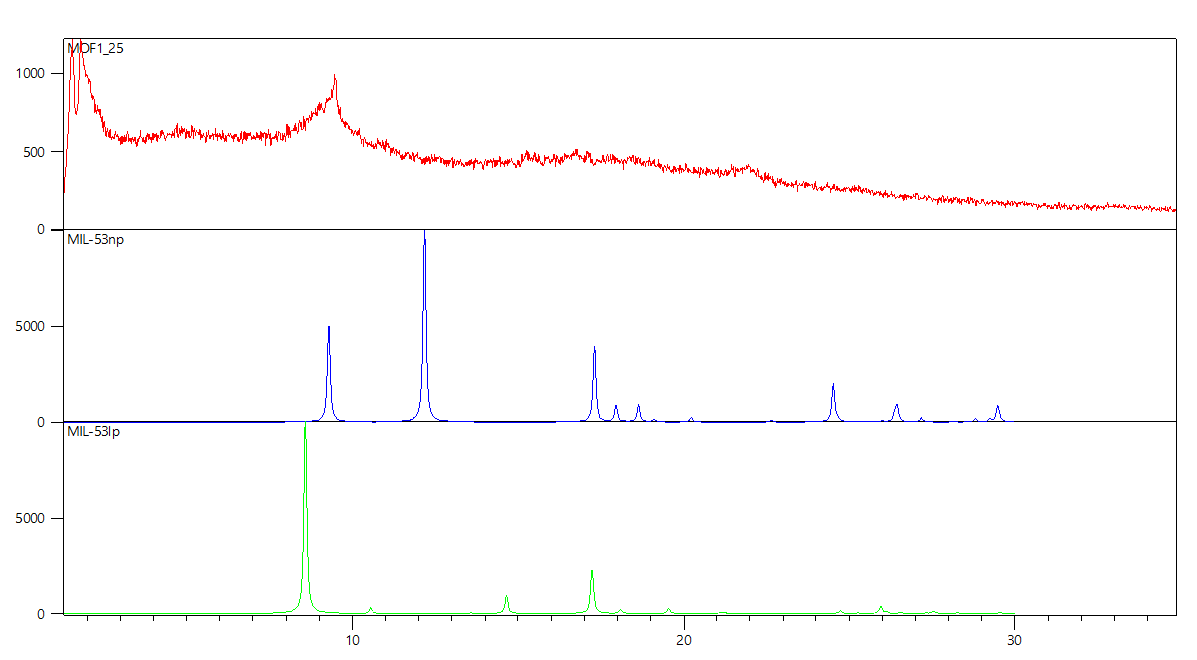
\includegraphics[scale=0.5]{MOF125ver.png}
    \caption{\textit{Es wird das Pulverdiffraktogramm von Al-MIL-53-H (rot) und die Referenzreflexe von MIL-53 narrow-pore (blau) Large-pore(grün) abgebildet}}
    \label{MOF125ver}
\end{figure}

\noindent
Aus Abbildung \ref{MOF125ver} lässt sich der Porentyp des hergestellten MOFs aufgrund der schwachen Reflexe nur schwer eindeutig bestimmen. 
Allerdings scheint eine bessere Übereinstimmung der Reflexe mit denen des Narrow-Pore-Typs vorzuliegen. 
Daher wird das hergestellte MOF Al-MIL-53-H dem Narrow-Pore-Typ zugeordnet.

\subsubsection{Porenanalyse Fe-MIL-53-H} \label{poreeisen}
In Abbildung \ref{MOF120ver} ist das Pulverdiffraktogramm von Fe-MIL-53-H zusammen mit den Referenzmustern dargestellt. Auch in diesem Fall ist eine eindeutige Zuordnung der Reflexe schwierig. 
Mithilfe der im Programm HighScore Plus generierten Peakliste (Reflexe bei 9.02°, 16.47° und 18.13°) lassen sich die Peaks jedoch dem eher dem Large-Pore-Typ zuordnen.
\newpage
\begin{figure}[!ht]
    \centering
    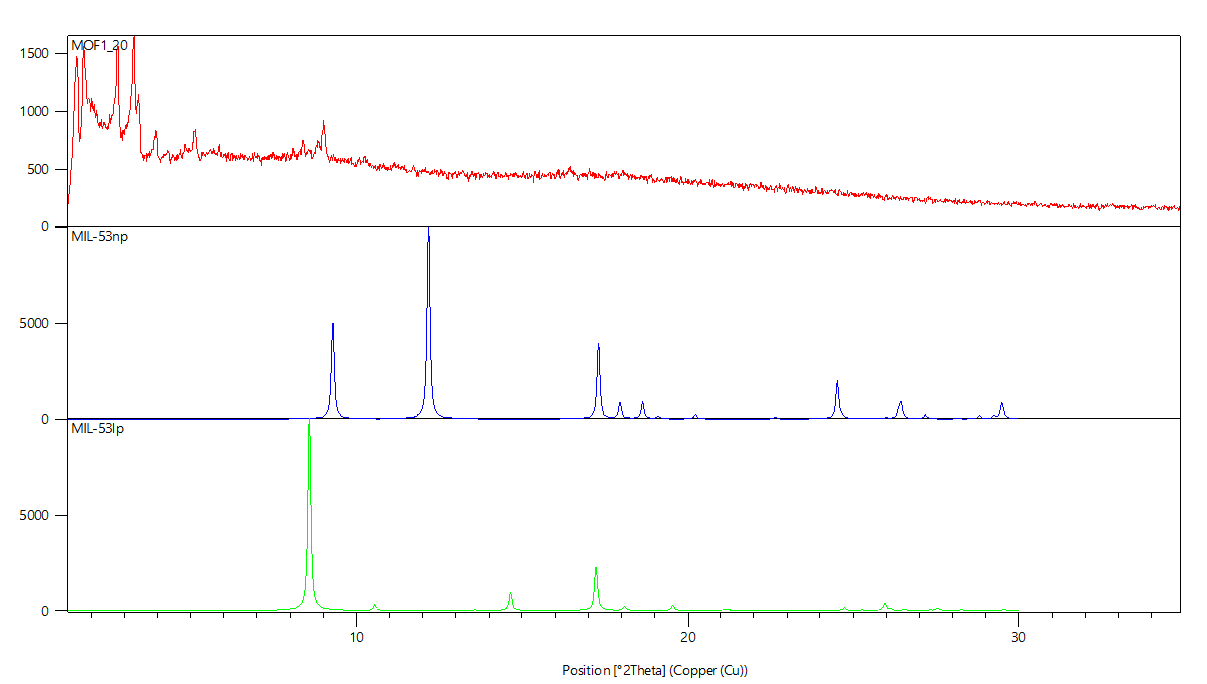
\includegraphics[scale=0.5]{MOF120ver.png}
    \caption{\textit{Es wird das Pulverdiffraktogramm von Fe-MIl-53-H (rot) und die Referenzreflexe von MIL-53 narrow-pore (blau) und Large-pore (grün) abgebildet}}
    \label{MOF120ver}
\end{figure}

\subsubsection{\texorpdfstring{Porenanalyse Al-MIL-53-NH$_2$}{Porenanalyse Al-MIL-53-NH2}}

In Abbildung \ref{MOF225ver} ist das Pulverdiffraktogramm von Al-MIL-53-NH$_2$ gemeinsam mit den Referenzmustern dargestellt. 
\begin{figure}[!h]
    \centering
    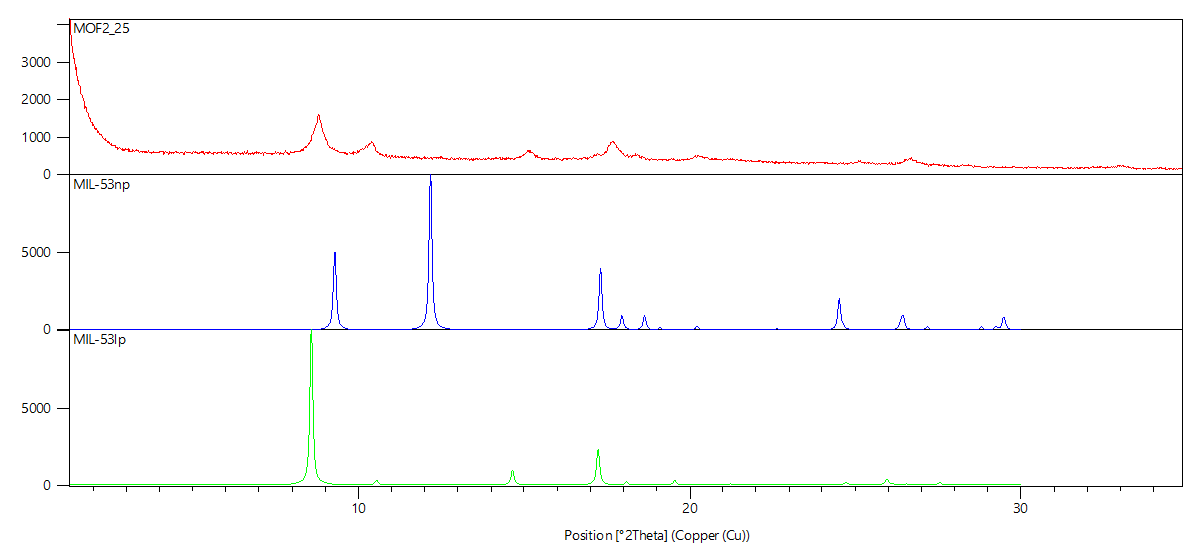
\includegraphics[scale=0.5]{MOF225ver.png}
    \caption{\textit{Es wird das Pulverdiffraktogramm von Al-MIl-53-NH$_2$ (rot) und die Referenzreflexe von MIL-53 narrow-pore (blau) und Large-pore (grün) abgebildet}}
    \label{MOF225ver}
\end{figure}
Aus Abbildung \ref{MOF225ver} geht hervor, dass Al-MIL-53-NH$_2$ in der Large-Pore-Konformation vorliegt. Dies lässt sich anhand der Übereinstimmung der gemessenen Reflexe mit denen des Large-Pore-Referenzmusters erkennen.

\newpage

\subsubsection{\texorpdfstring{Porenanalyse Fe-MIL-53-NH$_2$}{Porenanalyse Fe-MIL-53-NH2}} \label{poreeisenamino}
In Abbildung \ref{MOF220ver} ist das Pulverdiffraktogramm von Fe-MIL-53-NH$_2$ gemeinsam mit den Referenzmustern dargestellt. 

\begin{figure}[!h]
    \centering
    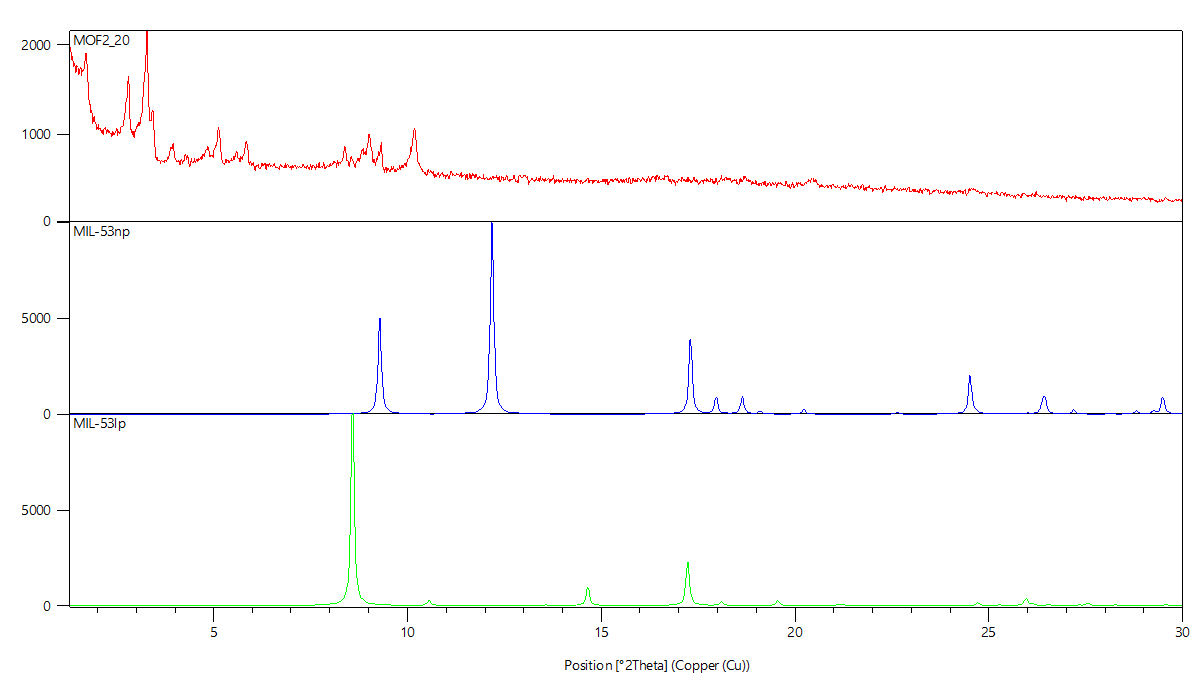
\includegraphics[scale=0.5]{MOF220ver.png}
    \caption{\textit{Es wird das Pulverdiffraktogramm von Al-MIl-53-NH$_2$ (rot) und die Referenzreflexe von MIL-53 narrow-pore (blau) und Large-pore (grün) abgebildet}}
    \label{MOF220ver}
\end{figure}
\noindent
Aus Abbildung \ref{MOF220ver} lässt sich nicht eindeutig erkennen, ob das MOF in der Narrow-Pore- oder in der Large-Pore-Konformation vorliegt. Die im Programm erstellte 
Peakliste liefert jedoch Hinweise auf die Large-Pore-Anordnung, da kleinere Reflexe bei 9.33°, 10.18°, 16.53° und 18.72° auftreten.
\newpage
\subsection{Iodkammer-Experiment}
Um zu überprüfen, ob das MOF Iod absorbieren kann, wird es mit gasförmigem Iod in Kontakt gebracht. Dies wird mithilfe von Rollgläsern erreicht.
Anschließend wird verglichen, wie sich das MOF verändert hat.
\subsubsection{Beobachtung Iodkammer Al-MIL-53-H}



\begin{figure}[h!]
    \centering
    \begin{subfigure}[b]{0.45\textwidth}
        \centering
        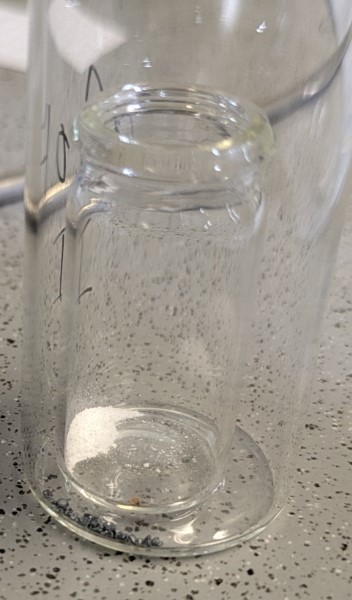
\includegraphics[width=0.7\textwidth]{MOF25Ivor.jpg}
        \caption{Al-MIL-53-H vor Kontakt mit gasförmigem Iod.}
        \label{VergleichMOF25Ivor}
    \end{subfigure}
    \hfill
    \begin{subfigure}[b]{0.45\textwidth}
        \centering
        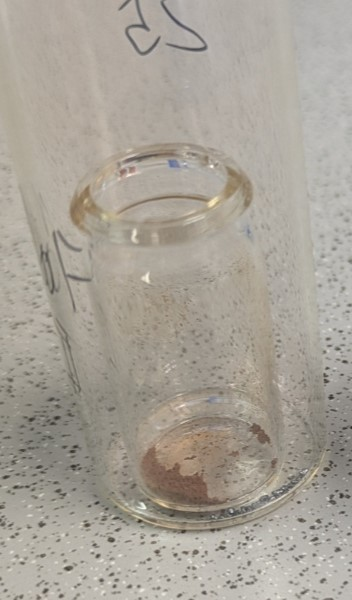
\includegraphics[width=0.7\textwidth]{MOF25Inach.jpg}
        \caption{Al-MIL-53-H nach Kontakt mit gasförmigem Iod.}
        \label{VergleichMOF25Inach}
    \end{subfigure}
    \caption{Vergleich von Al-MIL-53-H vor und nach der Behandlung mit gasförmigem Iod.}
    \label{VergleichMOF25I}
\end{figure}
\noindent
Aus Abbildung \ref{VergleichMOF25I} ist ersichtlich, dass der Al-MIL-53-H-MOF Iod aufnehmen kann. Dies zeigt sich an der Farbveränderung von Weiß zu Orangebraun.
\newpage

\subsubsection{Beobachtung Iodkammer Fe-MIL-53-H von Platz 21 durchgeführt}
\begin{figure}[!h]
    \centering
    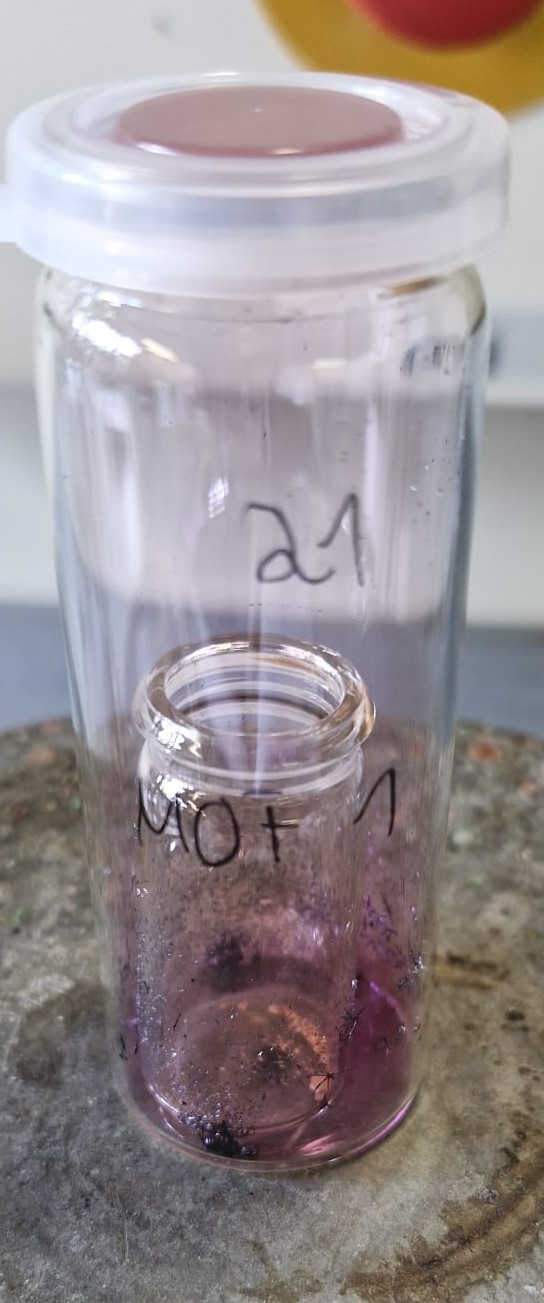
\includegraphics[width=0.25\linewidth]{MOF20I.jpg}
    \caption{Zeigt Fe-MIL-53-H, dass sich in der Iodkammer befindet.}
    \label{MOF20I}
\end{figure}

\noindent
Die Abbildung \ref{MOF20I} zeigt das MOF Fe-MIl-53-H in der Iodkammer. Leider wurde vergessen, ein Referenzbild aufzunehmen. Allerdings hat sich die Farbe nicht verändert. Somit kann Fe-MIL-53-H kein Iod aufnehmen.


\newpage
\subsubsection{\texorpdfstring{Beobachtung Iodkammer Al-MIL-53-NH$_2$}{Beobachtung Iodkammer Al-MIL-53-NH2}}

\begin{figure}[h!]
    \centering
    \begin{subfigure}[b]{0.48\textwidth}
        \centering
        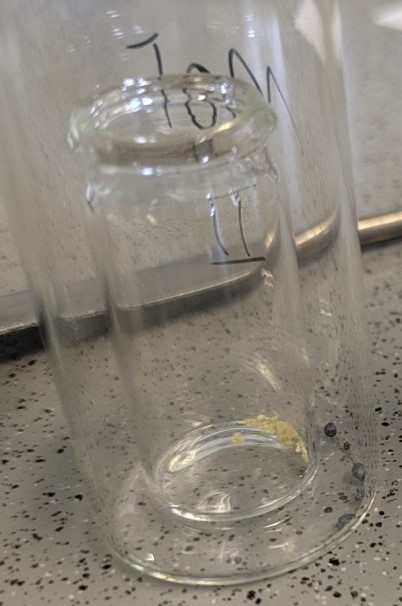
\includegraphics[width=0.7\textwidth]{MOF25IIvor.jpg}
        \caption{Al-MIL-53-NH$_2$ vor Kontakt mit gasförmigem Iod.}
        \label{VergleichMOF25IIvor}
    \end{subfigure}
    \hfill
    \begin{subfigure}[b]{0.48\textwidth}
        \centering
        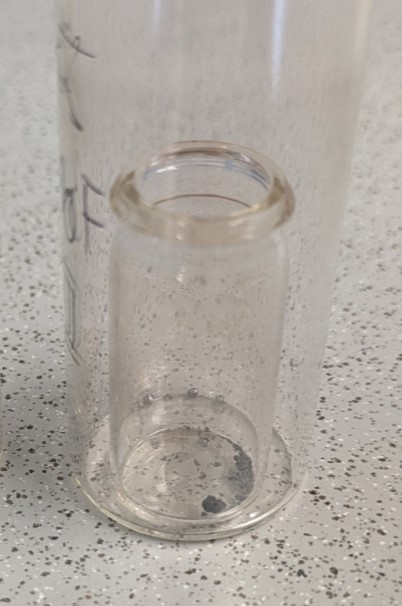
\includegraphics[width=0.7\textwidth]{MOF25IInach.jpg}
        \caption{Al-MIL-53-NH$_2$ nach Kontakt mit gasförmigem Iod.}
        \label{VergleichMOF25IInach}
    \end{subfigure}
    \caption{Vergleich von Al-MIL-53-NH$_2$ vor und nach der Behandlung mit gasförmigem Iod.}
    \label{VergleichMOF25II}
\end{figure}

\noindent
Aus Abbildung \ref{VergleichMOF25II} ist erkennbar, dass der Al-MIL-53-NH$_2$-MOF Iod aufnehmen kann. Dies zeigt sich an der Farbveränderung von Gelb zu Schwarz.


\newpage

\subsubsection{\texorpdfstring{Beobachtung Iodkammer Fe-MIL-53-NH$_2$ von Platz 20 durchgeführt}{Beobachtung Iodkammer Fe-MIL-53-NH2von Platz 20 durchgeführt}}

\begin{figure}[!h]
    \centering
    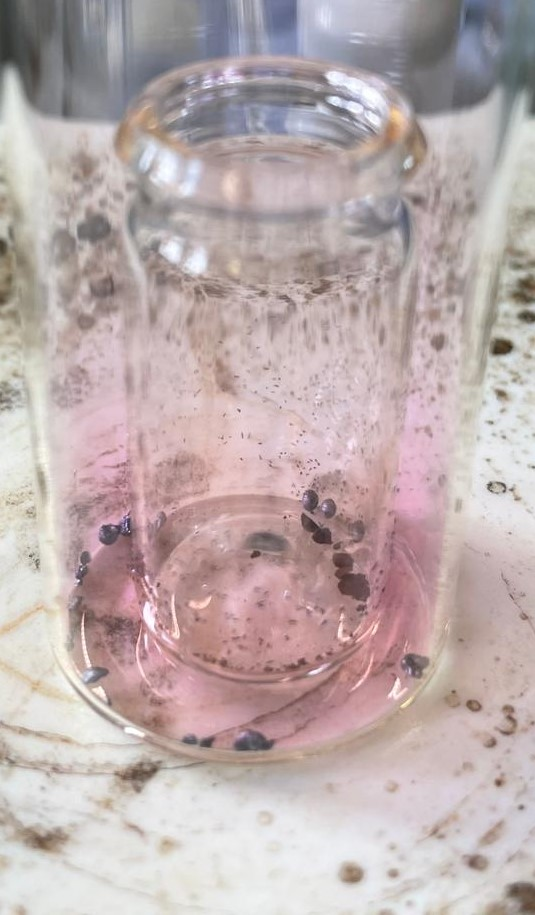
\includegraphics[width=0.25\linewidth]{MOF20II.jpg}
    \caption{Zeigt Fe-MIL-53-NH$_2$, dass sich in der Iodkammer befindet.}
    \label{MOF20II}
\end{figure}

\noindent
Die Abbildung \ref{MOF20II} zeigt das MOF Fe-MIL-53-NH$_2$ in der Iodkammer. Auch hier wurde leider kein Referenzbild aufgenommen. Dennoch war keine Farbveränderung zu beobachten, weshalb von keiner Iodeinlagerung ausgegangen werden kann.

\subsubsection{Erklärung des unteschiedlichen Verhalten bei der Einlagerung}
Aus den Iodkammer-Experimenten lässt sich schließen, dass die MOFs mit Aluminium als Metall Iod einlagern können, während der MOF aus Eisen dazu nicht fähig ist.

\noindent
Da die Linker der MOFs gleich sind und sich nur das Metallion unterscheidet, kann die Iodeinlagerung weder durch Physisorption (Van-der-Waals-Kräfte) noch durch Chemisorption, die von funktionellen Gruppen wie der Amin-Gruppe abhängt, erklärt werden.

\noindent
Daher ist als einziger Mechanismus nur die Diffusion des Gases in die Poren möglich. Dies lässt den Schluss zu, dass die Poren des Aluminium-MOFs größer sind als die des Eisen-MOFs. Beim Aluminium-MOF konnten die Iodmoleküle in das Netzwerk eindiffundieren und dadurch die Farbveränderung verursachen. Beim Eisen-MOF war dies nicht der Fall.
\newpage

\subsection{Physisorption des Eisen MOFs}
Da ursprünglich von allen vier MOFs die Physisorption gemessen werden sollte, jedoch nur eine geringe Probenmenge zur Verfügung stand, wurden von den Betreuern lediglich die Eisen-basierten MOFs erneut hergestellt und vermessen. Aus diesem Grund werden im vorliegenden Protokoll ausschließlich die Physisorptionsdaten der Eisen-MOFs betrachtet.

\noindent
Die entsprechenden Messdaten sind in Abbildung \ref{Physisorption} dargestellt.
\begin{figure}[!h]
    \centering
  \begin{subfigure}[b]{0.47\linewidth}
    \centering
    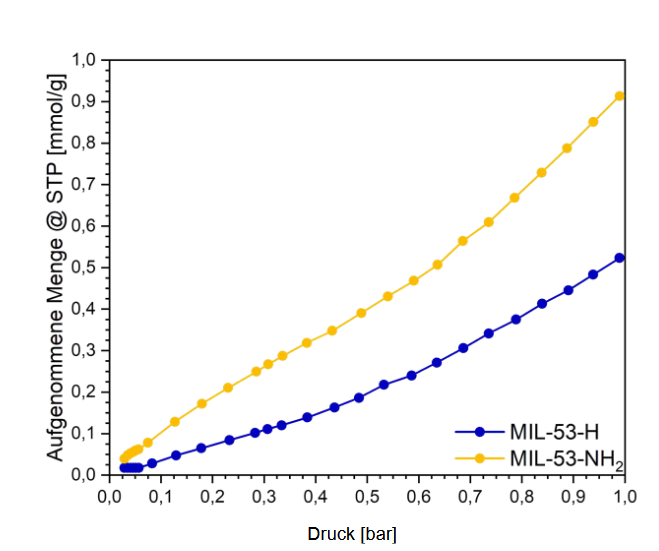
\includegraphics[width=\textwidth]{Phsyioganz.png}
    \caption{Physisorptionsisotherme im Bereich von 0.0 bis 1.0 bar.}
    \label{ganz}
    
  \end{subfigure}
   \begin{subfigure}[b]{0.47\linewidth}
    \centering
    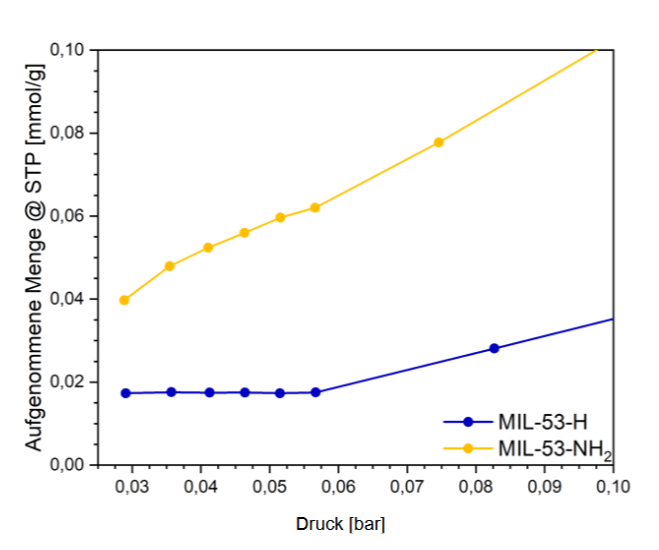
\includegraphics[width=\textwidth]{phsiozoom.png}
    \caption{Detailansicht im Druckbereich von 0.03 bis 0.10 bar.}
    \label{zoom}
    
  \end{subfigure}
  \caption{\ce{CO2}-Physisorption der Eisen-basierten MOFs bei 40 °C. Links ist die vollständige Isotherme dargestellt, rechts ein vergrößerter Ausschnitt im Niederdruckbereich.}
  \label{Physisorption}
\end{figure}

\noindent
Die Physisorptionsisothermen in Abbildung \ref{ganz} lassen sich nicht eindeutig nach der IUPAC-Klassi-fikation einordnen. Dennoch ist erkennbar, dass Fe-MIL-53-NH$_2$ das \ce{CO2} stärker physisorbiert als Fe-MIL-53-H. Dies liegt unter anderem am Quadrupolmoment, das sich zwischen der Aminogruppe (–NH$_2$) und dem \ce{CO2}-Molekül ausbilden kann.
Ein solcher spezifischer Wechselwirkungseffekt ist bei Fe-MIL-53-H, dem unfunktionalisierten MOF, nicht gegeben. Daher zeigt Fe-MIL-53-NH$_2$ eine höhere Affinität zur \ce{CO2}-Adsorption.

\noindent
In Abbildung \ref{zoom} ist zu erkennen, dass Fe-MIL-53-NH$_2$ bereits bei sehr niedrigen Drücken eine deutliche Physisorption von \ce{CO2} zeigt. Im Gegensatz dazu beginnt Fe-MIL-53-H erst bei einem höheren Druck (0.05668 bar) signifikant \ce{CO2} zu adsorbieren.
Dieser Unterschied lässt sich durch die strukturelle Flexibilität der MOFs erklären: Die Aminogruppe in Fe-MIL-53-NH$_2$ stabilisiert die großporige (Large-Pore) Konformation bereits im Ausgangszustand. Dadurch sind die Poren für \ce{CO2}-Moleküle frühzeitig zugänglich.
Fe-MIL-53-H hingegen liegt unter Startbedingungen in der engporigen (Narrow-Pore) Konformation vor, welche zunächst keinen Zugang für \ce{CO2} bietet. Erst ab einem Druck von etwa 0.05668 bar erfolgt ein struktureller Übergang zur großporigen Form, wodurch dann eine verstärkte Physisorption einsetzt.

\noindent
Im Abschnitt \ref{poreeisen} wurde Fe-MIL-53-H der Large-Pore Konformation zugeordnet. Ob diese Zuordnung korrekt ist, lässt sich jedoch nicht eindeutig beurteilen. Zwar wurde die Messung unter Normaldruck durchgeführt, allerdings betrug der Partialdruck von \ce{CO2} lediglich 0.0004 bar. Daher ist es unwahrscheinlich, dass \ce{CO2} allein für die Öffnung in die Large-Pore-Konformation verantwortlich war, möglicherweise war ein anderes Gas beteiligt.

\noindent
Im Gegensatz dazu wurde Fe-MIL-53-NH$_2$ im Abschnitt \ref{poreeisenamino} korrekt als Large-Pore identifiziert. Diese Zuordnung lässt sich durch die erhöhte Affinität zu \ce{CO2} und die bereits bei sehr niedrigen Drücken beobachtete Adsorption eindeutig bestätigen.

\newpage
\section{Zusammenfassung}
Im Rahmen des Versuchs wurden vier MOFs synthetisiert und anschließend hinsichtlich ihres Porentyps, ihrer Iodadsorption sowie ihrer \ce{CO2}-Physisorption untersucht. Die Ergebnisse zur Porenstruktur und zur Iodadsorption sind in Tabelle \ref{Zusammenfassung} zusammengefasst.
\begin{table}[!h]
    \caption{Zeigt das Verhalten der MOFs hinzüglich der Iodkammer und des Porentyps}
    \label{Zusammenfassung}
    \begin{tabular}{|>{\columncolor{lightgray}\centering\arraybackslash}p{0.3\linewidth}|>{\centering\arraybackslash}p{0.3\linewidth}|>{\centering\arraybackslash}p{0.3\linewidth}|}
        \hline
        \rowcolor{gray}
        MOF&Porentyp&Adsorbiert Iod\\
        \hline
         Al-MIL-53-H & Narrow-Pore & Ja \\
        \hline
        Fe-MIL-53-H & Large-Pore / Narrow-Pore & Nein \\
        \hline
        Al-MIL-53-NH$_2$ & Large-Pore & Ja \\
        \hline
        Fe-MIL-53-NH$_2$ & Large-Pore & Nein \\
        \hline
    \end{tabular}



\end{table}

\noindent
Aus Tabelle \ref{Zusammenfassung} lässt sich ablesen, dass die Fe-basierten MOFs kein Iod einlagern können, während die Al-basierten MOFs dazu in der Lage sind. Zudem zeigt sich, dass die Einführung einer Aminogruppe den Porentyp beeinflusst: Sie bewirkt eine Umwandlung von einem Narrow-Pore- zu einem Large-Pore-System.

\noindent
\noindent
Bei der \ce{CO2}-Physisorption fiel auf, dass der Amino-MOF eine deutlich höhere Adsorption zeigt als der entsprechende MOF ohne Aminogruppe. Dieses Verhalten lässt sich auf die durchgehende Large-Pore-Struktur sowie auf die spezifische Wechselwirkungen zwischen der Aminogruppe und den \ce{CO2}-Molekülen zurückführen.


\newpage
\section{Literaturverzeichnis}
\printbibliography


\end{document}